\documentclass[11pt]{article}
\usepackage[utf8]{inputenc}
\usepackage{amsmath, amssymb, amsthm}
\usepackage{geometry}
\usepackage{tikz}
\usetikzlibrary{angles,quotes}
\geometry{a4paper, margin=2cm}

\title{\textbf{KTO Matematika Juni 2015}\\Soal dan Pembahasan}
\author{Idham Muqoddas\\[1ex] \small{Sumber: ktom-tomi.or.id}}
\date{}

\begin{document}

\maketitle

\section*{Soal Bagian A: Isian}
\begin{enumerate}
    \item Pada sebuah papan catur $8 \times 8$, setiap barisnya diberi label bilangan 1 sampai 8 dan setiap kolomnya diberi label huruf $A$ sampai $H$. Hitunglah banyaknya kotak pada papan catur yang berada pada baris berlabel bilangan prima dan kolom berlabel huruf vokal.
    
    \item Tentukan semua bilangan bulat $n$ sehingga $\frac{n+3}{n-1}$ merupakan bilangan bulat.
    
    \item Sebanyak 2015 koin dibagi menjadi 10 tumpukan. Tentukan banyak koin minimum pada tumpukan yang paling besar.
    
    \item Diketahui bilangan bulat positif $n$ merupakan hasil jumlah 2015 bilangan bulat berurutan. Tentukan nilai terkecil yang mungkin untuk $n$.
    
    \item Diberikan segi-8 beraturan $ABCDEFH$. Tentukan besar sudut $\angle BCH$.
    
    \item Diberikan sebuah segitiga dengan panjang sisi $BC = 20, CA = 24$, dan $AB = 12$. Titik $D$ pada segmen $BC$ dengan $BD = 5$. Lingkaran luar dari segitiga $ABD$ memotong $CA$ di $E$. Hitung panjang $DE$.
    
    \item Diberikan dua buah dadu. Dadu pertama berbentuk kubus dengan sisi berangka 1 hingga 6 dan peluang muncul setiap sisi adalah sama. Dadu kedua berbentuk limas dengan sisi berangka 1 hingga 4 dan peluang muncul setiap sisi adalah sama. Kedua buah dadu dilemparkan bersamaan. Berapakah peluang jumlah bilangan yang muncul genap?
    
    \item Misalkan $a > b > c > d$ bilangan real sehingga $a + b + c + d = 1$ dan $ab + bc + cd + da = -1$. Tentukan nilai $a - b + c - d$.
    
    \item Pada Sae Games 2015, setiap keping emas bernilai 4 poin, perak bernilai 2 poin dan perunggu bernilai 1 poin. Negara Anggrek mendapatkan poin 420. Total medali yang diraih negara Anggrek adalah 150. Misalkan $N$ menyatakan banyaknya medali emas yang mungkin diperoleh negara Anggrek jika diketahui informasi tersebut. Tentukan banyaknya nilai yang mungkin untuk $N$.
    
    \item Diberikan jajar genjang $ABCD$ yang luasnya 4 satuan. Misalkan $E$ titik tengah $CD$ dan $F$ titik tengah $AB$. Garis $AE$ memotong garis $DF$ di $K$. Garis $AC$ memotong garis $DF$ dan $BE$ berturut-turut di $L$ dan $M$. Hitunglah luas $EKLM$.
    
    \item Misalkan $x_1, x_2, \dots, x_{2015}$ menyatakan akar-akar dari persamaan $x^{2015} + 2x^{2014} + 3x^{2013} + \dots + 2015x + 2016 = 0$. Tentukan nilai $\sum_{n=0}^{2015} \sum_{k=1}^{2015} (x_k)^n$.
    
    \item Diberikan segilima siklis $ABCDE$ yang kelilingnya 36 satuan. Segitiga $ABD$ merupakan segitiga sama sisi dengan panjang sisi 10 satuan. Diketahui $CE = 8$ satuan. Jika $F$ merupakan titik potong $AC$ dan $BE$, hitunglah panjang $FA + FB$.
    
    \item Tentukan semua bilangan prima $p$ sedemikian sehingga terdapat bilangan bulat $n$ yang memenuhi $n(n - 1)(n - 2)(n - 3) - 1678 \le p^2 \le n(n - 1)(n - 2)(n - 3) - 1656$.
    
    \item Empat kakak beradik dengan nama Andi, Bayu, Candika, Danang, Ellena, Fanny, Gina, Hani sedang bermain catur. Diketahui bahwa: (1) Ellena bermain dengan kakaknya Gina (2) Hani bermain dengan kakaknya Ellena (3) Fanny bermain dengan Andi (4) Bayu bermain dengan adiknya Candika (5) Candika bermain dengan adiknya Andi. Sebut lawan bermain Gina sebagai $X$. Tentukan saudara dari $X$.
    
    \item Diketahui $a, b \in \mathbb{R}$ yang memenuhi $a + \frac{1}{a + 2015} = b - 4030 + \frac{1}{b - 2015}$ dan $|a - b| > 5000$. Tentukan nilai dari $\frac{ab}{2015} - a + b$.
    
    \item Diberikan sebuah segitiga dengan panjang sisi $BC = 9, CA = 10$, dan $AB = 11$. Misalkan titik $I$ adalah pusat lingkaran dalam dari segitiga $ABC$. Misalkan pula $I_B$ adalah pusat lingkaran singgung luar segitiga $ABC$ terhadap $B$ yang menyinggung segmen $CA$ dan sinar garis $AB$ dan $BC$. Hitunglah panjang $II_B$.
    
    \item Suatu tumpukan kartu terdiri dari 2016 kartu yang dinomori 1, 2, \dots, 2016. Tumpukan kartu ini dikocok sehingga urutan awal kartu-kartu tidak diketahui. Sebuah permainan dimainkan yang melakukan dua langkah berikut bergantian hingga semua kartu habis: (1) kartu paling atas dipindahkan ke paling bawah tumpukan, (2) kartu paling atas dikeluarkan dari tumpukan. Setelah semua kartu keluar dari tumpukan, ternyata urutan kartu yang dikeluarkan adalah 1, 2, \dots, 2016. Tentukan kartu mana yang berada di atas tumpukan pada urutan awal kartu tersebut.
    
    \item Diberikan sebuah fungsi $f : \mathbb{N} \to \mathbb{Q}$ dengan $f(1) = \frac{3}{2}$ dan $f(x + y) = \left(1 + \frac{y}{x + 1}\right) f(x) + \left(1 + \frac{x}{y + 1}\right) f(y) + x^2y + xy + xy^2$. Tentukan nilai $f(20)$.
    
    \item Misalkan $(a, b, c)$ merupakan pasangan bilangan asli yang memenuhi persamaan $a^2 + 2b^2 + 4c^2 = k(a + b + c)$. Carilah nilai $k$ terkecil sehingga persamaan tersebut memiliki minimal dua solusi.
    
    \item Misalkan $a_i$ adalah koefisien dari $x^i$ pada penjabaran $(1 + 3x)^{2015}$ untuk setiap bilangan bulat $i$ dengan $0 \le i \le 2015$. Carilah banyak nilai $k$ di mana $0 \le k \le 2014$ sedemikian sehingga $a_k < a_{k+1}$.
    
    \item Misalkan $x, y$, dan $z$ bilangan real yang memenuhi $x + y + z = 0$ dan $x^2 + y^2 + z^2 = 6$. Carilah nilai maksimum dari $|(x - y)(y - z)(z - x)|$.
\end{enumerate}

\section*{Soal Bagian B: Esai}
\begin{enumerate}
    \item Diberikan segiempat $PQRS$ sedemikian sehingga: (1) segitiga $PSR$ merupakan segitiga siku-siku dengan $\angle PSR = 90^\circ$, (2) segitiga $PRQ$ merupakan segitiga siku-siku dengan $\angle PRQ = 90^\circ$. Diketahui $|PS| = 12, |SR| = 9$, dan $|PQ| = 25$. 
    \begin{enumerate}
        \item Tentukan luas segiempat $PQRS$.
        \item Tentukan panjang diagonal $|QS|$.
    \end{enumerate}
    
    \item Barisan $\{a_n\}$ dan $\{b_n\}$ diberikan dengan definisi $a_1 = 625$ dan $a_n = 625^{a_{n-1}}$ serta $b_1 = 5$ dan $b_n = 5^{b_{n-1}}$ untuk setiap bilangan asli $n > 1$. Tentukan bilangan asli $k$ terkecil sehingga $b_k > a_{625}$.
    
    \item Pada papan catur berukuran $4 \times 4$ akan diletakkan sebanyak 7 buah kuda identik. Tentukan banyak cara meletakkannya sehingga tidak ada dua buah kuda yang saling menyerang.
\end{enumerate}

\newpage
\section*{Pembahasan Bagian A}
\begin{enumerate}
    \item Baris prima ada 4 ($2, 3, 5, 7$) dan kolom vokal ada 2 ($A, E$). Banyak kotak = $4 \times 2 = \boxed{\boxed{8}}$.
    \item Ubah $\frac{n+3}{n-1} = 1 + \frac{4}{n-1}$. Syarat $n-1 \mid 4 \implies n-1 \in \{\pm1, \pm2, \pm4\}$. Nilai $n = \boxed{\boxed{-3, -1, 0, 2, 3, 5}}$.
    \item Misalkan $x_1 \le x_2 \le \dots \le x_{10}$ adalah banyak koin di tiap tumpukan. Agar $x_{10}$ sekecil mungkin, bagikan koin seimbang mungkin. $2015 = 10 \times 201 + 5$. Maka dapat dibuat 5 tumpukan berisi 202 koin, dan sisanya 201 koin. Nilai minimum tumpukan terbesar adalah \boxed{\boxed{202}}.
    \item Misalkan ke-2015 bilangan tersebut rata-ratanya $a$. Hasil jumlahnya $n = 2015a$. Agar $n$ bulat positif dan terkecil, nilai $a$ (median barisan) bulat positif terkecil yang mungkin, yaitu $a=1$. Maka $n = 2015 \times 1 = \boxed{\boxed{2015}}$.
    \item Sudut interior segi-8 beraturan adalah $135^\circ$. Busur $BH$ memuat dua sisi, sehingga sudut pusat $\angle BOH = 90^\circ$. Maka besar sudut keliling $\angle BCH = \frac{90^\circ}2 = \boxed{\boxed{45^\circ}}$.
    
    \begin{center}
    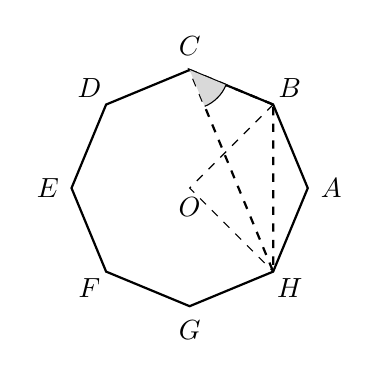
\begin{tikzpicture}[scale=1.5]
        \foreach \i/\l in {1/A, 2/B, 3/C, 4/D, 5/E, 6/F, 7/G, 8/H} {
            \coordinate (\l) at ({45*(\i-1)}:1);
            \node at ({45*(\i-1)}:1.2) {$\l$};
        }
        \draw[thick] (A)--(B)--(C)--(D)--(E)--(F)--(G)--(H)--cycle;
        \draw[thick, dashed] (B)--(C)--(H)--cycle;
        \draw[dashed] (B)--(0,0)--(H);
        \node[below] at (0,0) {$O$};
        \pic [draw, fill=gray!30, angle radius=0.5cm] {angle = H--C--B};
    \end{tikzpicture}
    \end{center}
    \item Karena $A,B,D,E$ siklis, $\triangle CDE \sim \triangle CAB$.  \begin{align*}\frac{DE}{AB} &= \frac{CD}{CA}\\[4pt] &= \frac{15}{24} \\[4pt]&= \frac58 \\ DE &= 12 \times \frac58 \\&= \boxed{\boxed{7.5}}\end{align*}
    
    \begin{center}
    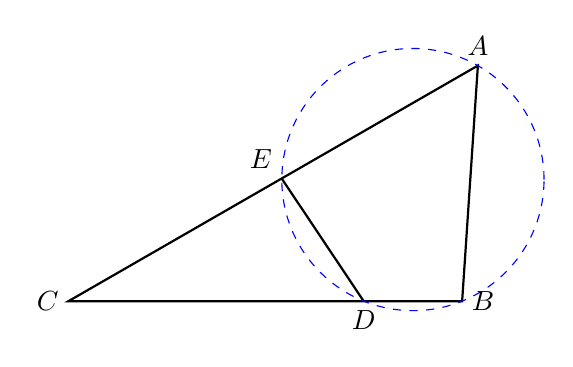
\begin{tikzpicture}[scale=0.25]
        \coordinate (C) at (0,0);
        \coordinate (B) at (20, 0);
        \coordinate (A) at (20.8, 11.97);
        \coordinate (D) at (15, 0);
        \coordinate (E) at (10.83, 6.24);
        
        \draw[thick] (C) -- (A) -- (B) -- cycle;
        \draw[thick] (E) -- (D);
        \draw[dashed, blue] (17.5, 6.18) circle (6.66);
        
        \node[left] at (C) {$C$}; \node[above] at (A) {$A$}; \node[right] at (B) {$B$};
        \node[above left] at (E) {$E$}; \node[below] at (D) {$D$};
    \end{tikzpicture}
    \end{center}

    \item Peluang jumlah genap terjadi jika keduanya ganjil atau keduanya genap. Dadu 1 (ganjil $\frac12$, genap $\frac12$), dadu 2 (ganjil $\frac12$, genap $\frac12$). \\[4pt] Peluang = $\left(\frac12 \times \frac12\right) + \left(\frac12 \times \frac12\right) = \frac12$.
    \item Perhatikan bahwa $$ab+bc+cd+da = (a+c)(b+d) = -1$$ Misal $x=a+c$ dan $y=b+d$. Maka $x+y=1, xy=-1$.  $$a-b+c-d = x-y = \sqrt{(x+y)^2 - 4xy} = \sqrt{1^2 - 4(-1)} = \sqrt{5}$$.
    \item Emas (4), perak (2), perunggu (1). Sistem persamaan: $$\begin{cases} e+p+r&=150\\4e+2p+r&=420\end{cases}$$ Eliminasi $r$ menghasilkan \begin{align*}3e+p&=270 \\ p &= 270-3e\end{align*} Karena $p \ge 0, r = 2e-120 \ge 0$, diperoleh rentang $60 \le e \le 90$. Banyak nilai $e$ (atau $N$) ada 31.
    \item Karena $AF \parallel DE$ dan $AF = \frac{1}{2}AB = \frac{1}{2}CD = DE$, maka segiempat $AFED$ adalah jajargenjang. Diagonal-diagonalnya $AE$ dan $DF$ saling membagi dua sama panjang di $K$, sehingga $K$ adalah titik tengah $AE$ dan $AK = \frac{1}{2} AE$. Di $\triangle ADC$, $AE$ adalah garis berat. Karena $F$ membagi $AB$ sama panjang, garis $DF$ memotong $AC$ di titik $L$ yang merupakan titik berat $\triangle ABD$. Akibatnya, $AL = \frac{1}{3} AC$. Dengan simetri yang sama, $M$ adalah titik berat $\triangle BCD$, sehingga $CM = \frac{1}{3} AC$. Hal ini berarti $L$ dan $M$ membagi diagonal $AC$ menjadi tiga bagian sama panjang ($AL = LM = MC$), yang juga menyiratkan $AL = \frac{1}{2} AM$.\\
    Pada $\triangle AEM$, karena $AK = \frac{1}{2} AE$ dan $AL = \frac{1}{2} AM$, maka $\triangle AKL \sim \triangle AEM$ dengan rasio sisi $1:2$. \\Luas $\triangle AEM = \frac{AM}{AC} \times \text{Luas } \triangle AEC = \frac{2}{3} \times (\frac{1}{2} \text{Luas } \triangle ADC) = \frac{2}{3} \times 1 = \frac{2}{3}$.\\[4pt]
    Luas $\triangle AKL = (\frac{1}{2})^2 \times \text{Luas } \triangle AEM = \frac{1}{4} \times \frac{2}{3} = \frac{1}{6}$.\\
    Maka Luas $EKLM = \text{Luas } \triangle AEM - \text{Luas } \triangle AKL = \frac{2}{3} - \frac{1}{6} = \boxed{\boxed{\frac{1}{2}}}$.
    
    \begin{center}
    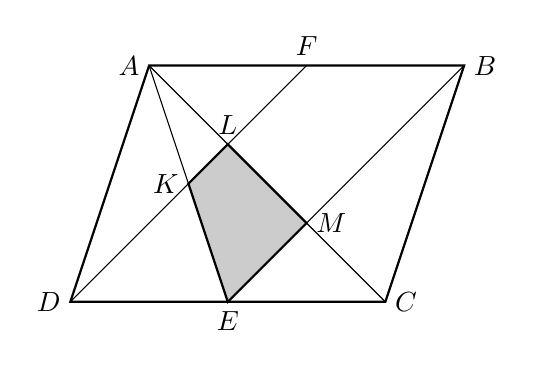
\begin{tikzpicture}[scale=2]
        \coordinate (D) at (0,0); \coordinate (C) at (2,0);
        \coordinate (A) at (0.5,1.5); \coordinate (B) at (2.5,1.5);
        \coordinate (E) at (1,0); \coordinate (F) at (1.5,1.5);
        \draw[thick] (A)--(B)--(C)--(D)--cycle;
        \draw (A)--(E); \draw (D)--(F);
        \draw (A)--(C); \draw (B)--(E);
        \node[left] at (A) {$A$}; \node[right] at (B) {$B$};
        \node[right] at (C) {$C$}; \node[left] at (D) {$D$};
        \node[below] at (E) {$E$}; \node[above] at (F) {$F$};
        % K is AE intersect DF
        \coordinate (K) at (intersection of A--E and D--F);
        % L is AC intersect DF
        \coordinate (L) at (intersection of A--C and D--F);
        % M is AC intersect BE
        \coordinate (M) at (intersection of A--C and B--E);
        \draw[fill=gray!40, thick] (E)--(K)--(L)--(M)--cycle;
        \node[left] at (K) {$K$}; \node[above] at (L) {$L$}; \node[right] at (M) {$M$};
    \end{tikzpicture}
    \end{center}
    \item Misal $S=x^{2015} + 2x^{2014} + 3x^{2013} + \dots + 2015x + 2016$, maka
\begin{align*}xS&=x^{2016} + 2x^{2015} + 3x^{2014} + \dots + 2015x^2 + 2016x\\
S&=x^{2015} + 2x^{2014} + 3x^{2013} + \dots + 2015x + 2016\qquad-\\ \hline\\[-14pt]
(x-1)S&=x^{2016}+x^{2015}+x^{2014} +\dots +x-2016 \\
0&=x\left(x^{2015}+x^{2014}+\dots+x+1\right)-2016\\
x\left(\frac{x^{2016}-1}{x-1}\right)&=2016\\[4pt]
\frac{x^{2016}-1}{x-1}&=2016\cdot\frac1x
\end{align*}
\begin{align*}\sum_{k=1}^{2015} \sum_{n=0}^{2015} x_k^n &= \sum_{k=1}^{2015} \frac{x_k^{2016}-1}{x_k-1}\\[4pt]
&=\sum_{k=1}^{2015}2016\cdot\frac1{x_k}\\[4pt]
&=2016\sum_{k=1}^{2015}\frac1{x_k}\\[4pt]
&=2016\left(\frac{-a_1}{a_0}\right)\\[4pt]
&=2016\left(\frac{-2015}{2016}\right)\\
&=\boxed{\boxed{-2015}} \end{align*}
    \item Teorema Ptolemy pada ABCD \begin{align*}
BD\cdot AC&=AD\cdot BC+AB\cdot CD\\
 10 AC &= 10 BC + 10 CD \\ AC &= BC+CD\end{align*} Demikian pula $BE = DE+EA$. Total keliling tanpa $AB$ adalah $26$, maka $AC+BE=26$. Dapat dibuktikan $\triangle FCE \sim \triangle FAB$, sehingga rasio sisinya $$\frac{CE}{AB} = \frac8{10} = \frac45$$ Akibatnya $FC = \frac{4}{5}FB$ dan $FE = \frac{4}{5}FA$. \begin{align*}AC+BE&=26\\  (FA+FC)+(FB+FE)&=26 \\ \frac{9}{5}(FA+FB) &= 26 \\ FA+FB &= \frac{130}9\end{align*}
    
    \begin{center}
    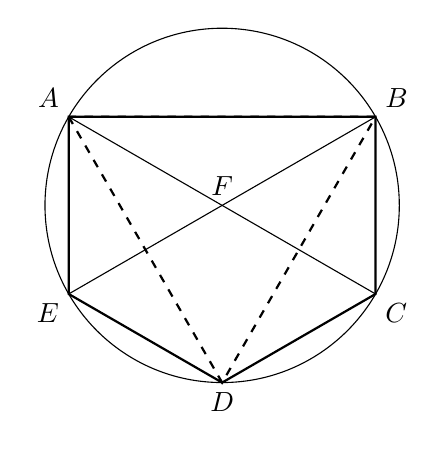
\begin{tikzpicture}[scale=1.5]
        \draw (0,0) circle (1.5);
        \coordinate (A) at (150:1.5);
        \coordinate (B) at (30:1.5);
        \coordinate (D) at (270:1.5);
        \coordinate (C) at (330:1.5);
        \coordinate (E) at (210:1.5);
        \draw[thick] (A)--(B)--(C)--(D)--(E)--cycle;
        \draw[thick, dashed] (A)--(D)--(B)--cycle;
        \draw (A)--(C); \draw (B)--(E);
        \coordinate (F) at (intersection of A--C and B--E);
        \node[above left] at (A) {$A$}; \node[above right] at (B) {$B$};
        \node[below right] at (C) {$C$}; \node[below] at (D) {$D$}; \node[below left] at (E) {$E$};
        \node[above] at (F) {$F$};
    \end{tikzpicture}
    \end{center}
    \item Tulis bentuk sebagai $(n^2-3n+1)^2 - 1679 \le p^2 \le (n^2-3n+1)^2 - 1657$. Misalkan $x = n^2-3n+1$. Kita cari prima $p$ yang berjarak tertentu dari bilangan kuadrat. Bentuk ekuivalen: $1657 \le (x-p)(x+p) \le 1679$. Dengan menguji faktor yang memenuhi $(x-p)$ dan $(x+p)$ paritas sama, kita temukan kasus $(x-p)=3 \implies (x+p) = 557$ dan diperoleh nilai prima $p=277$.
    \item Anggap orang-orang berasal dari 4 keluarga berbeda dengan pasangan Kakak-Adik. Dari keterangan: A bersaudara dengan H, C bersaudara dengan E, B bersaudara dengan G, dan sisanya D bersaudara dengan F. Pertandingan yang terjadi adalah A vs F, B vs E, C vs H, D vs G. Lawan G (Gina) adalah D (Danang), saudara dari D adalah Fanny (F).
    \item Misalkan $x=a+2015, y=b-2015$. Persamaan menjadi $x+1/x = y+1/y \implies (x-y)(1 - 1/(xy)) = 0$. Karena $|a-b|>5000$, maka $x \neq y$, sehingga $xy = 1$. Dengan menjabarkan $(a+2015)(b-2015)=1$, diperoleh $ab - 2015a + 2015b = 2015^2 + 1$. Maka nilai $\frac{ab-2015a+2015b}{2015} = \frac{2015^2+1}{2015} = 2015 + \frac{1}{2015}$.
    \item Pusat lingkaran dalam $I$ dan singgung luar $I_B$ terletak di garis bagi $\angle B$. Lingkaran berdiameter $II_B$ melalui $A, C$, berpusat di $M$ (titik tengah busur $AC$). Maka $II_B = 2AM = 4R\sin(B/2)$. Substitusi jari-jari lingkaran luar $R = b/(2\sin B)$, diperoleh $II_B = b / \cos(B/2)$. Dengan Aturan Cosinus, $\cos B = 17/33 \implies \cos(B/2) = 5/\sqrt{33}$. Maka $II_B = 10 / (5/\sqrt{33}) = 2\sqrt{33}$.
    
    \begin{center}
    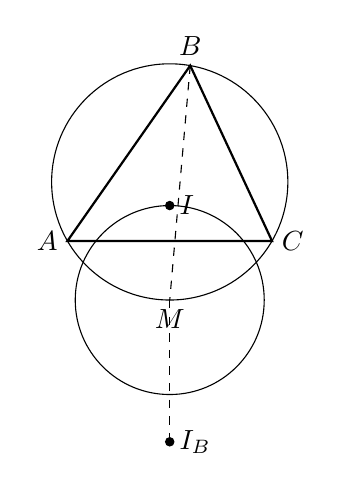
\begin{tikzpicture}[scale=1.5]
        \coordinate (A) at (210:1);
        \coordinate (C) at (330:1);
        \coordinate (B) at (80:1);
        \draw (0,0) circle (1);
        \draw[thick] (A)--(B)--(C)--cycle;
        \node[above] at (B) {$B$}; \node[left] at (A) {$A$}; \node[right] at (C) {$C$};
        \coordinate (M) at (270:1);
        \node[below] at (M) {$M$};
        
        \draw[dashed] (B) -- (M);
        \coordinate (I) at (0, -0.2); 
        \coordinate (Ib) at (0, -2.2);
        \draw[fill=black] (I) circle (1pt) node[right]{$I$};
        \draw[fill=black] (Ib) circle (1pt) node[right]{$I_B$};
        \draw[dashed] (M) -- (Ib);
        \draw (M) circle (0.8);
    \end{tikzpicture}
    \end{center}
    \item Proses pembuangan akan selalu menyisakan elemen yang berada pada pola indeks deret ganjil/genap tertentu (simulasi Josephus variasi). Dengan melacak posisi kartu yang pertama ditaruh di bawah dari tumpukan asli, perhitungan deret pembuangan akan menunjukkan ia terbuang pada putaran ke-1985. Maka kartu teratas awal bernomor 1985.
    \item Bagikan persamaan dengan $(x+y+1)$, dan definisikan $g(x) = \frac{f(x)}{x+1}$. Didapatkan $g(x+y) - g(x) - g(y) = xy$. Bentuk umum fungsi yang memenuhi adalah $g(x) = cx + \frac{x^2}{2}$. Dari $f(1)=3/2$, diperoleh $g(1)=3/4 \implies c=1/4$. Jadi $g(x) = \frac{2x^2+x}{4}$. $f(20) = 21 \times g(20) = 21 \times 205 = 4305$.
    \item Kuadratkan sempurna ruas kiri: $4(a-k/2)^2 + 2(2b-k/2)^2 + (4c-k/2)^2 = 7k^2/4$. Substitusi nilai asli dan minimumkan dengan uji $k$ kelipatan 2 terkecil. Saat $k=6$, kita mendapat persamaan $2(a-3)^2 + (2b-3)^2 + \frac{1}{2}(4c-3)^2 = \frac{63}{2}$. Terdapat solusi $(6,1,2)$ dan $(6,2,2)$. Jawaban minimum $k=6$.
    \item Nilai $a_k = \binom{2015}{k} 3^k$. Ketaksamaan $a_k < a_{k+1}$ setara dengan $\frac{1}{2015-k} < \frac{3}{k+1} \implies k+1 < 6045 - 3k \implies 4k < 6044$. Karena batas atas asli adalah $k = 1510$, dari $0$ sampai $1510$ ada 1511 nilai $k$.
    \item Berdasarkan teorema Vieta, $x,y,z$ adalah akar polinomial $t^3 + qt - r = 0$, di mana $q = -3$ dari nilai $x^2+y^2+z^2=6$. Ekstremum $|(x-y)(y-z)(z-x)|$ adalah akar dari diskriminan polinomial tersebut $\Delta = -4q^3 - 27r^2 = 108 - 27r^2$. Maksimum terjadi saat $r=0$, sehingga nilainya $\sqrt{108} = 6\sqrt{3}$.
\end{enumerate}

\section*{Pembahasan Bagian B}
\begin{enumerate}
    \item \textbf{Segiempat $PQRS$}
    
    Perhatikan $\triangle PSR$ siku-siku di $S$. Menurut Teorema Pythagoras, $PR = \sqrt{12^2+9^2} = 15$. 
    Pada $\triangle PRQ$ siku-siku di $R$, $RQ = \sqrt{25^2-15^2} = 20$.
    \begin{enumerate}
        \item Luas $PQRS$ = Luas $\triangle PSR$ + Luas $\triangle PRQ$ = $\frac{1}{2} (12)(9) + \frac{1}{2} (15)(20) = 54 + 150 = 204$.
        \item Tarik garis tegak lurus dari $Q$ ke perpanjangan $SR$, sebut titik potongnya $T$. Perhatikan $\triangle PSR$ dan $\triangle RTQ$. Karena $\angle PRQ = 90^\circ$ (dan titik $S, R, T$ segaris lurus), maka $\angle PRS + \angle QRT = 180^\circ - 90^\circ = 90^\circ$. Pada $\triangle PSR$ yang siku-siku di $S$, juga berlaku $\angle PRS + \angle SPR = 90^\circ$. Hal ini menyiratkan $\angle QRT = \angle SPR$. Karena kedua segitiga tersebut siku-siku ($\angle S = \angle T = 90^\circ$), maka menurut prinsip Sudut-Sudut, $\triangle QTR \sim \triangle RSP$.
        Perbandingan kesebangunan ini menghasilkan perbandingan sisi: $\frac{QT}{RS} = \frac{TR}{SP} = \frac{QR}{RP} = \frac{20}{15} = \frac{4}{3}$.
        Disubstitusikan nilainya: $\frac{QT}{9} = \frac{4}{3} \implies QT = 12$, dan $\frac{TR}{12} = \frac{4}{3} \implies TR = 16$.
        Panjang total $ST = SR + TR = 9 + 16 = 25$.
        Dengan Teorema Pythagoras pada $\triangle QTS$ yang siku-siku di $T$, panjang diagonal $QS = \sqrt{ST^2 + QT^2} = \sqrt{25^2 + 12^2} = \sqrt{625+144} = \sqrt{769}$.
    \end{enumerate}
    
    \vspace{1ex}
    \begin{center}
    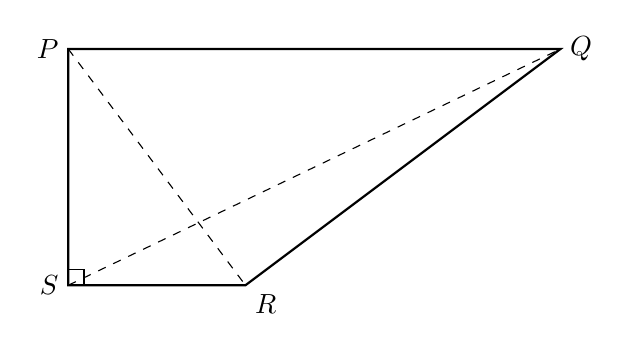
\begin{tikzpicture}[scale=0.25]
        \coordinate (S) at (0,0);
        \coordinate (R) at (9,0);
        \coordinate (P) at (0,12);
        \coordinate (Q) at (25,12);
        
        \draw[thick] (P) -- (Q) -- (R) -- (S) -- cycle;
        \draw[dashed] (P) -- (R);
        \draw[dashed] (S) -- (Q);
        
        \node[left] at (S) {$S$};
        \node[below right] at (R) {$R$};
        \node[left] at (P) {$P$};
        \node[right] at (Q) {$Q$};
        
        \draw (0,0.8) -- (0.8,0.8) -- (0.8,0);
    \end{tikzpicture}
    \end{center}
    \vspace{1ex}
    
    \item \textbf{Barisan $a_n$ dan $b_n$}
    
    Dapat dibuktikan dengan induksi bahwa nilai $a_n$ memiliki struktur tumpukan pangkat dengan tinggi $n$ dan puncaknya $4 \cdot 5^4$, sedangkan $b_n$ puncaknya 5. Berlaku $a_n < b_{n+1}$ dan $a_n > b_n$ untuk setiap $n \ge 1$. Oleh karena $b_{625} < a_{625} < b_{626}$, maka nilai bilangan asli $k$ terkecil adalah $626$.
    
    \item \textbf{Papan Catur}
    
    Papan catur diwarnai selang-seling hitam putih. Agar tidak saling menyerang, ke-7 kuda harus ditempatkan sedemikian rupa meminimalkan kotak aman yang dikurangi pada warna berlawanan. Jika semua kuda 1 warna: $H=7, P=0$ ($\binom{8}{7}=8$ cara) dan $H=0, P=7$ ($\binom{8}{7}=8$ cara).
    Jika $H=6, P=1$, kuda putih harus di pojok (2 posisi), menyisakan 6 posisi hitam yang tidak terserang (yang terpaksa harus ditempati ke-6 kuda). Kombinasi $H=1, P=6$ memberikan hal simetris (2 cara). Solusi H dan P tidak mungkin memiliki formasi lain karena persilangan serangan akan memakan porsi aman di atas batas sisa 7 kuda.
    Total cara = $8 + 8 + 2 + 2 = 20$.
    
\end{enumerate}

\end{document}
